\documentclass{article}
% bibliography setup
\usepackage{natbib}
\bibliographystyle{apalike}  % abbrvnat
\setcitestyle{authoryear,open={(},close={)}} %Citation-related commands
% makes color citations
\usepackage[colorlinks=true,urlcolor=blue,citecolor=red,linkcolor=red,bookmarks=true]{hyperref}
% images
\usepackage{graphicx}
\graphicspath{ {./images/} }

% hypter parameter setup
\usepackage{hyperref}
% for table setup
\usepackage{multirow}

% for pseudo code
\usepackage{algorithm}
\usepackage{algpseudocode}

% to highlight lines of code, as per: https://tex.stackexchange.com/questions/149779/how-can-i-colourfuly-highlight-some-lines-of-an-algorithm-using-algorithm2e
\usepackage{xcolor}
\def\HiLi{\leavevmode\rlap{\hbox to \hsize{\color{yellow!50}\leaders\hrule height .8\baselineskip depth .5ex\hfill}}}


\title{Improved Sequential Hypothesis Testing with
``Enhanced Precision Is The Goal"}
\date{\today}
\author{Eyal A. Kazin}

\begin{document}
\maketitle

\input precision_goal_abstract

\section{Introduction}
\input precision_goal_introduction

\subsection{Contributions}

\subsubsection{Paper Structure}
The paper is organized as follows.
In the Methods section we describe three (four if Frequentist?)
stop criteria as well as the setup to test on synthetic deichotomous data.
In the Results section we present the results of the synthetic data analysis as well as analytical analysis.
In the Discussion section we discuss the implications of the results (Reword this).
In the Conclusion section we summarize the findings and suggest future directions (Reword this).


\section{Methods}

\input precision_goal_methods


\section{Results}

Figure \ref{fig:iterations} presents the results of the a cherry picked fair coin
experiment ($\theta_{\rm true}=0.5$). It was chosen to highlight potential stark
different outcomes of the three stop criteria. For comparison note that the posteriors
shown in Figure \ref{fig:posteriors} are three iterations of this figure.
(TB footnote: 1 - provide the sequence, 2 - reference to JK figure number)

As we can see from both figures at iteration 126 the credible interval (95\% HDI posterior) of HDI+ROPE is fully
outside of the ROPE making it confidently, though incorrectly, reject $\theta_{\rm null}$.

The Precision is the Goal stop criterion is met at iteration 598, where the credible
interval width
subpasses the precision goal of 0.08. Since the credible interval straddles the ROPE
the decision is inconclusive.

The Enhanced Precision is the Goal stop criterion is met at iteration 804, where the credible interval
meets both criterions: narrower than 0.08 precision goal and fully within the ROPE.
This results in correctly accepting $\theta_{\rm null}$.

\begin{figure}[h!]
  \centering
  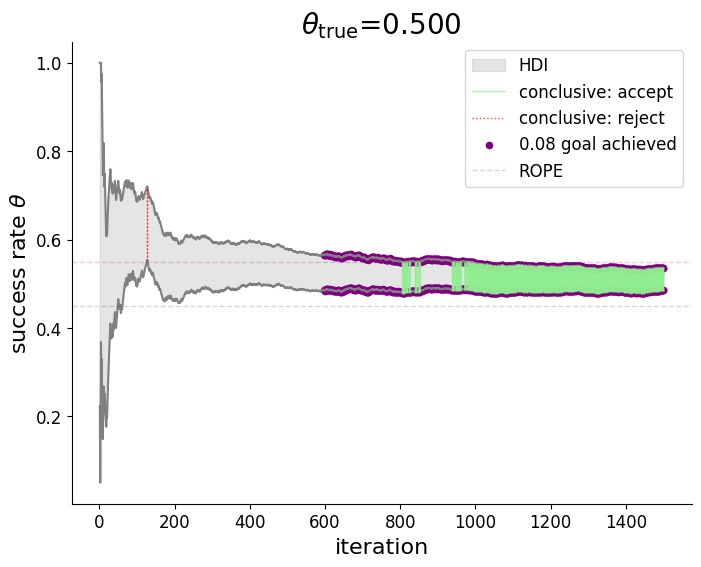
\includegraphics[width=1\textwidth]{cherry_iterations.png}
  \caption{Cherry picked fair coin sample demonstrating the varied outcomes by
  stop criterion mechanism. The vertical axis is the cumulative success rate
  at each iteration (horizontal axis).
  The gray band is the 95\% HDI of the posterior at each iteration.
  The highlighted iterations indicate where stop criterion trigger conditions are met:
  red dashed lines is when  $\theta_{\rm null}$ may be rejected, green solid lines
  is when he $\theta_{\rm null}$ may be accepted. Purple dots on the 95\% HDI boundaries
  indicated when the precision goal is achieved. Note that the posteriors of Figure \ref{fig:posteriors}
  are slices of this figure: HDI+ROPE is the the first red dashed line (iteration 126),
  Precision is the Goal is the first purple dot (598), and Enhanced Precision is the Goal is the second purple dot (598)
  is the first green line (804). The ROPE boundaries is represented by the dashed lines.
  }
  \label{fig:iterations}
\end{figure}

In Figure \ref{fig:fair_iter_vs_rate} we explore how representative this cherry picked example is by exploring
the outcomes of $M=500$ experiments. (TK Ref JK figure number being additional information to his histograms).

\begin{figure}[h!]
  \centering
  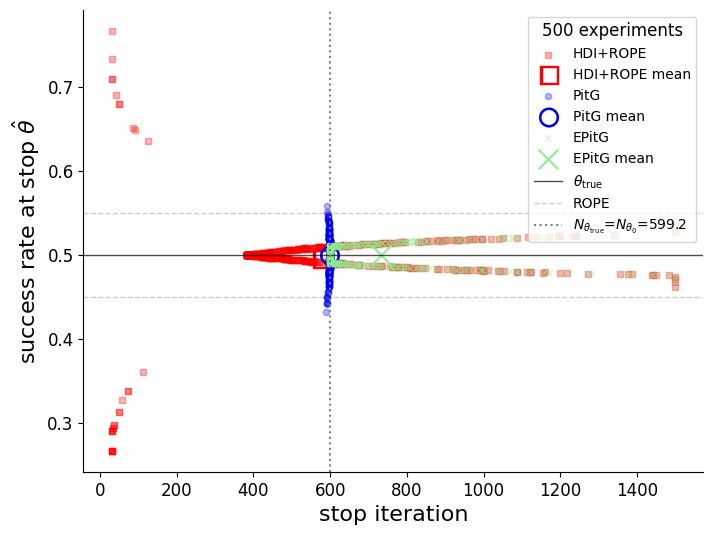
\includegraphics[width=1\textwidth]{fair_experiments_iter_vs_rate.png}
  \caption{Small symbols are individual experiment outcomes. Large are experiments
  mean values. When using HDI+ROPE as the stop criterion results in the red squares.
  Precision is the Goal as the criterion results in the blue circles
  and the Enhanced PitG as the green Xs. $\theta_{\rm true}$ is the solid line and
  the ROPE is the dashed lines. TK: analytical results
  }
  \label{fig:fair_iter_vs_rate}
\end{figure}

The large symbols that represent the 500 expeirment outcome means 
(large red square, blue circle and X as per legend) show
that on average all methods are unbiased outcomes.

That said, HDI+ROPE yields 6\% False Positives (red squares).
(Note that if we relax the minimum sample size ($N_{\rm min}=0$) the FPR increases to TK\%).
Precision is the Goal stops around iteration ~590 but is 61\% inconclusive (blue circles).
For conclusiveness of these 61\%, the Enhanced PitG requires more sampling (green Xs)
resulting in only 1.6\% inconclusive outcomes by final iteration of $N_{\rm max}=1,500$.

TK table with numerical summaries. Add to explanation value above

% organise the following into a latex table, please
% accept	reject	conclusive	inconclusive	stop_iter_mean	stop_iter_std	success_rate_mean	success_rate_std
% hdi_rope	0.928	0.06	0.988	0.012	576.590	280.975530	0.495168	0.050294
% pitg	0.390	0.00	0.390	0.610	598.254	1.389008	0.499376	0.019967
% epitg	0.984	0.00	0.984	0.016	732.242	210.538168	0.499801	0.012725

\begin{table}[h!]\label{tab:bah}
  \begin{center}
  \begin{tabular}{c|c|c|c|c|c|c|c|c}
    \hline
    Algorithm & Accept & Reject & Conclusive & Inconclusive & mean stop & stop std & $\hat{\theta}$ & $\sigma_{\hat{\theta}}$\\
    \hline
    HDI+ROPE & 0.928 & 0.06 & 0.988 & 0.012 & 576.6 & 281 & 0.4952 & 0.0502 \\
    PitG & 0.390 & 0.00 & 0.390 & 0.610 & 598.3 & 1.4 & 0.4994 & 0.01997 \\
    ePitG & 0.984 & 0.00 & 0.984 & 0.016 & 732.2 & 210 & 0.4998 & 0.0127\\
    \hline
  \end{tabular}
  \caption{Numerical summaries of 500 experiments of three stop criteria. Accept
  is the fraction of experiments which results in acceptence of $\theta_{\rm null}$,
  and similar for Reject, Conclusive and Inconclusive. The mean stop is the average}
\end{center}
\end{table}


\begin{table}[h!]\label{tab:table1}
  \begin{center}
    \begin{tabular}{c|c|c|c}
      \textbf{Test Algorithm } & \textbf{Pre Survey} & \textbf{Stop Criterion} &  \textbf{Decision Criterion}\\
      \hline
      HDI + ROPE & $N_\mathrm{min}$  & \multicolumn{2}{c}{\multirow{1}{*}{HDI within/outside ROPE?}}  \\
      Precision is the Goal & Goal & Precision $<$ Goal? & HDI within/outside ROPE? \\
      Enhanced Precision is the Goal & Goal& \multicolumn{2}{c}{\multirow{1}{*}{(Precision $<$ Goal?) \& (HDI within/outside ROPE?)}}  \\
    \end{tabular}
    \caption{A high level comparison between the test algorithms.
    The merged cells mean Stop and Decision criteria are simultaneous.
    Otherwise multi-step.
    }
  \end{center}
\end{table}

Noteworhty insights from the figure are:
\begin{itemize}
  \item HDI + ROPE confidently accepting
  \item HDI + ROPE gap
  \item PitG barreir
  \item Enhanced ePitG barreir and extending same as HDI + ROPE
\end{itemize}

\section{Discussion}

\section{Conclusion}

\section{Useful Equations}
\input precision_goal_useful_equations

\section{Submission Instructions}

Methods Paper—maximum word count: 6500
Methods Papers present an advance likely to make major impact in one or more applied
fields. While theory (e.g. theorems concerning statistical or
learning-theoretic properties) are welcome, this is not essential, but intuition and
understanding of why the method works is important.
We are also very open to theory in a broader sense including examples and conjectures.
Generally, we would expect empirical results to demonstrate effectiveness.
However, in cases where the extent of methodological/conceptual innovation is large
enough, results themselves may be illustrative and need not be of immediate high impact
in any particular applied domain.

Each piece should include:

Unstructured Abstract—maximum word count: 250
Keywords—maximum of 6 and minimum of 5
May include tables and figures—no limit
May include the following back matter sections:
Acknowledgements
Author contributions (with CRediT details)
Conflicts of interest
Funding
Must include the following:
Data availability
References—no limit
Each submission must contain the following sections and use these terms as the first
level section headers: Introduction, Methods, Results, Discussion and Conclusion
(Discussion and Conclusion may be combined).

{\bf Resources}

\href{https://academic.oup.com/rssdat/pages/general-instructions}{RSS Instructions} 

\href{https://academic.oup.com/pages/authoring/books/preparing-your-manuscript/working-in-latex}{RSS Working in \LaTeX}.

\bibliography{references.bib}

\end{document}